\documentclass{beamer}
\usetheme{CambridgeUS}
\usepackage[utf8]{inputenc}
\usepackage{listings}
\usepackage{tikz}
\usepackage{graphicx}
\usepackage{blkarray}
\usepackage{xcolor}
\usepackage[normalem]{ulem}
\usepackage{verbatim}

\graphicspath{ {res/} } 
 
%Information to be included in the title page:
\title{The Adventures of Alice (and Bob) in Wonderland}
\author{Henk Bierlee \and Nodari Kankava}
\institute{Uppsala University}
\date{Spring 2019}
 
% TODO footer is clipping

\definecolor{mygreen}{rgb}{0,0.6,0}
\definecolor{mygray}{rgb}{0.5,0.5,0.5}
\definecolor{mymauve}{rgb}{0.58,0,0.82}

\definecolor{regiongreen}{RGB}{134, 196, 134}
\definecolor{regionpurple}{RGB}{194, 134, 196}
\definecolor{regionorange}{RGB}{255, 150, 0}
\definecolor{regionblue}{RGB}{0, 204, 255}

\lstset{ 
  backgroundcolor=\color{white},   % choose the background color; you must add \usepackage{color} or \usepackage{xcolor}; should come as last argument
  basicstyle=\footnotesize,        % the size of the fonts that are used for the code
  breakatwhitespace=false,         % sets if automatic breaks should only happen at whitespace
  breaklines=true,                 % sets automatic line breaking
  commentstyle=\color{mygreen},    % comment style
  deletekeywords={...},            % if you want to delete keywords from the given language
  escapeinside={\%*}{*)},          % if you want to add LaTeX within your code
  extendedchars=true,              % lets you use non-ASCII characters; for 8-bits encodings only, does not work with UTF-8
  frame=single,	                   % adds a frame around the code
  columns=flexible,
  keepspaces=true,                 % keeps spaces in text, useful for keeping indentation of code (possibly needs columns=flexible)
  keywordstyle=\color{blue},       % keyword style
  language=C++,                 % the language of the code
  numbers=none,                    % where to put the line-numbers; possible values are (none, left, right)
  rulecolor=\color{black},         % if not set, the frame-color may be changed on line-breaks within not-black text (e.g. comments (green here))
  showspaces=false,                % show spaces everywhere adding particular underscores; it overrides 'showstringspaces'
  showstringspaces=false,          % underline spaces within strings only
  showtabs=false,                  % show tabs within strings adding particular underscores
  stepnumber=2,                    % the step between two line-numbers. If it's 1, each line will be numbered
  stringstyle=\color{mymauve},     % string literal style
  tabsize=2,	                   % sets default tabsize to 2 spaces
  %title=\lstname                   % show the filename of files included with \lstinputlisting; also try caption instead of title
}

 
\begin{document}

% \setbeamertemplate{caption}{%
% \begin{beamercolorbox}[wd=.5\paperwidth, sep=.2ex]{block body}\insertcaption%
% \end{beamercolorbox}%
% }

% \setbeamertemplate{caption}{\raggedright\insertcaption\par}


 
\frame{\titlepage}
 
\begin{frame}{Problem statement}

\begin{figure}
    \centering
    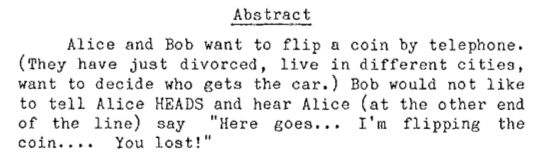
\includegraphics{blum-abstract}
    \caption{Abstract from \emph{COIN FLIPPING BY TELEPHONE: A PROTOCOL FOR SOLVING IMPOSSIBLE PROBLEMS} by M. Blum (1981)}
    \label{fig:blum-abstract}
\end{figure}

\end{frame}

\begin{frame}{A classical solution:  llock-box analogy}

\begin{enumerate}
    \item Alice writes down her call (heads/tails) on paper and locks it in a box with her key
    \item Alice sends the box (but not the key) to Bob
    \item Bob tosses the coin and reports outcome to Alice
    \item Alice reveals who won and sends her key to Bob so he can verify Alice's claim
\end{enumerate}

Relies on the assumption that Bob cannot open the box, in other words: \emph{computational hardness}.

% TODO maybe skip this whole slide?

\end{frame}

\begin{frame}{Presentation overview}

\begin{itemize}
    \item \sout{Problem statement}
    \vfill
    \item Recap: behaviour of polarised photons
    \vfill
    \item Remote quantum coin-toss protocol
    \vfill
    \item Advantages and disadvantages
    \vfill
    \item Questions
    \vfill
\end{itemize}

\end{frame}

\begin{frame}{Behaviour of polarised photons}



\end{frame}

\begin{frame}{Quantum Coin-Toss Protocol}
\begin{itemize}
    \item Alice encodes a random bit-string with a randomly chosen base and sends them to Bob
    \item Bob randomly chooses a base for each photon and fills corresponding measurement table and makes a guess.
    \item Alice reveals the correct base and sends original bit-string over classic communication channel
    \item Bob verifies that Alice didn't cheat by comparing bit-string to corresponding measurement table
\end{itemize}
\end{frame}

\begin{frame}{Impossibility of Cheating}
\begin{itemize}
    \item Possibility of correct guess is exactly 1/2.
    \item Alice has to provide all the measurement results.
\end{itemize}
\end{frame}

\begin{frame}{Disadvantages}
\begin{itemize}
    \item Need for quantum hardware
    \item Einstein-Podolsky-Rosen effect
\end{itemize}
\end{frame}

\begin{frame}{Questions}

\end{frame}
 

\end{document}


    % \begin{itemize}
    %     \item \begin{verbatim}
    %          0 1 0 1 0 0 
    %         \end{verbatim}
    %     % \item \begin{verbatim}
    %     %         RECTILINEAR
    %     %     \end{verbatim}
    % \end{itemize}